
\documentclass[sigconf]{acmart}

\setcopyright{none}
\settopmatter{printacmref=false}
\renewcommand\footnotetextcopyrightpermission[1]{}
\usepackage{pdfpages}
%%
%% end of the preamble, start of the body of the document source.
\begin{document}
\pagestyle{empty}
%%
%% The "title" command has an optional parameter,
%% allowing the author to define a "short title" to be used in page headers.
\title{\textbf{OrcaLink: Modeling Potential Social Ties in Southern Resident Killer Whales}}

%%
%% The "author" command and its associated commands are used to define
%% the authors and their affiliations.
%% Of note is the shared affiliation of the first two authors, and the
%% "authornote" and "authornotemark" commands
%% used to denote shared contribution to the research.

\author{Aung Htut}
\email{amhtut@uvic.ca}
\affiliation{%
  \institution{University of Victoria}
   \country{Canada}
}
\author{Bowen Zhang}
\email{bowenzhang1@uvic.ca}
\affiliation{%
  \institution{University of Victoria}
   \country{Canada}
}

%%
%% The abstract is a short summary of the work to be presented in the
%% article.
\begin{abstract}
  Southern Resident killer whales (SRKWs) have multiple types of relationships, including pod membership, matrilineal kinship, and social associations.
Genealogical and relationship information must be considered together with sighting and encounter information to comprehensively query familial and social relationships among individuals.
Therefore, this project develops a data model that integrates relationship and sighting information to explore and identify not only observed associations but also potential association candidates based on shared associations and kinship. The project repository is available on
\href{https://github.com/CSC501-OrcaLink/OrcaLink}{GitHub}.
\end{abstract}

\maketitle



\section{Introduction}

Southern Resident killer whales (SRKWs) generally travel in matrilineal family groups but also form social associations \cite{ellis2017}. Encounter and photo-identification records have been collected since 1976 \cite{cwrhistory}. Individual records describe whales' identities, demographic information, and matrilineal relationships \cite{orcaConservancy}, while sighting records identify individuals observed together, along with dates and locations \cite{thompson2026dryad}.

Family membership and observed associations represent different types of relationships. Although previous studies have investigated demographic and social association data \cite{ellis2017}, examining individual records alone makes it difficult to jointly query kinship, repeated co-sightings, and indirect connections across multiple encounters. OrcaLink aims to integrate these relationships into a data model that supports queries about both direct and indirect associations among individuals.

\section{Motivation}

SRKWs are listed as endangered under the Endangered Species Act (ESA) \cite{epaSRKW}. Following the death of SRKW L95 in 2016, to which a tag-related infection contributed, NOAA suspended its satellite-tagging program for review \cite{noaaTagging}. Our project uses publicly available sighting records~\cite{thompson2026dryad} to investigate associations among individuals.

Observational records are incomplete, and direct co-sightings alone may not capture indirect connections. Examining encounter records individually also makes it difficult to explore familial relationships and changes in associations across multiple sightings.

Previous research has examined the relationship between social network position and mortality risk in SRKWs \cite{ellis2017}, highlighting the scientific relevance of social associations. By integrating demographic information and historical sightings, OrcaLink aims to help marine biology researchers explore familial and social relationships, identify potential associations, and estimate which individuals may be observed together in the future.

\subsection{Motivating Example}
L87 (Onyx), a member of L pod, has been repeatedly observed with J pod, including documented observations alongside J pod individuals such as J49 and J37\cite{cwr2019mar22}. On December 17, 2019, L87 was traveling with individuals from J and L pods when individuals from K pod and other members of L pod joined them, forming a large group of whales from different pods\cite{cwr2019dec17}.

Which individuals have been repeatedly observed with L87, and how have these relationships changed over time? Does L87 serve as a potential social bridge connecting individuals from different pods? Furthermore, which whales are indirectly connected to L87 through shared associates, even if they have never been directly observed together?

OrcaLink calculates co-sighting affinity between L87 and other individuals and explores connection paths between different pods and potential social bridges. A separate prediction model then estimates the likelihood of co-sightings between L87 and particular individuals.

\section{Team Justification}

Our team brings complementary strengths in data integration, representation, and analysis. Aung will focus on data-source investigation, whale ID, genealogy, and encounter integration, data provenance, preprocessing, and SQL/SPARQL query development and validation. Bowen will focus on relational schema implementation, RDF/OWL mapping, and SQL/SPARQL development. All members will collaborate on schema design, integration, and overall validation.

\bibliographystyle{ACM-Reference-Format}
\bibliography{References}
\clearpage
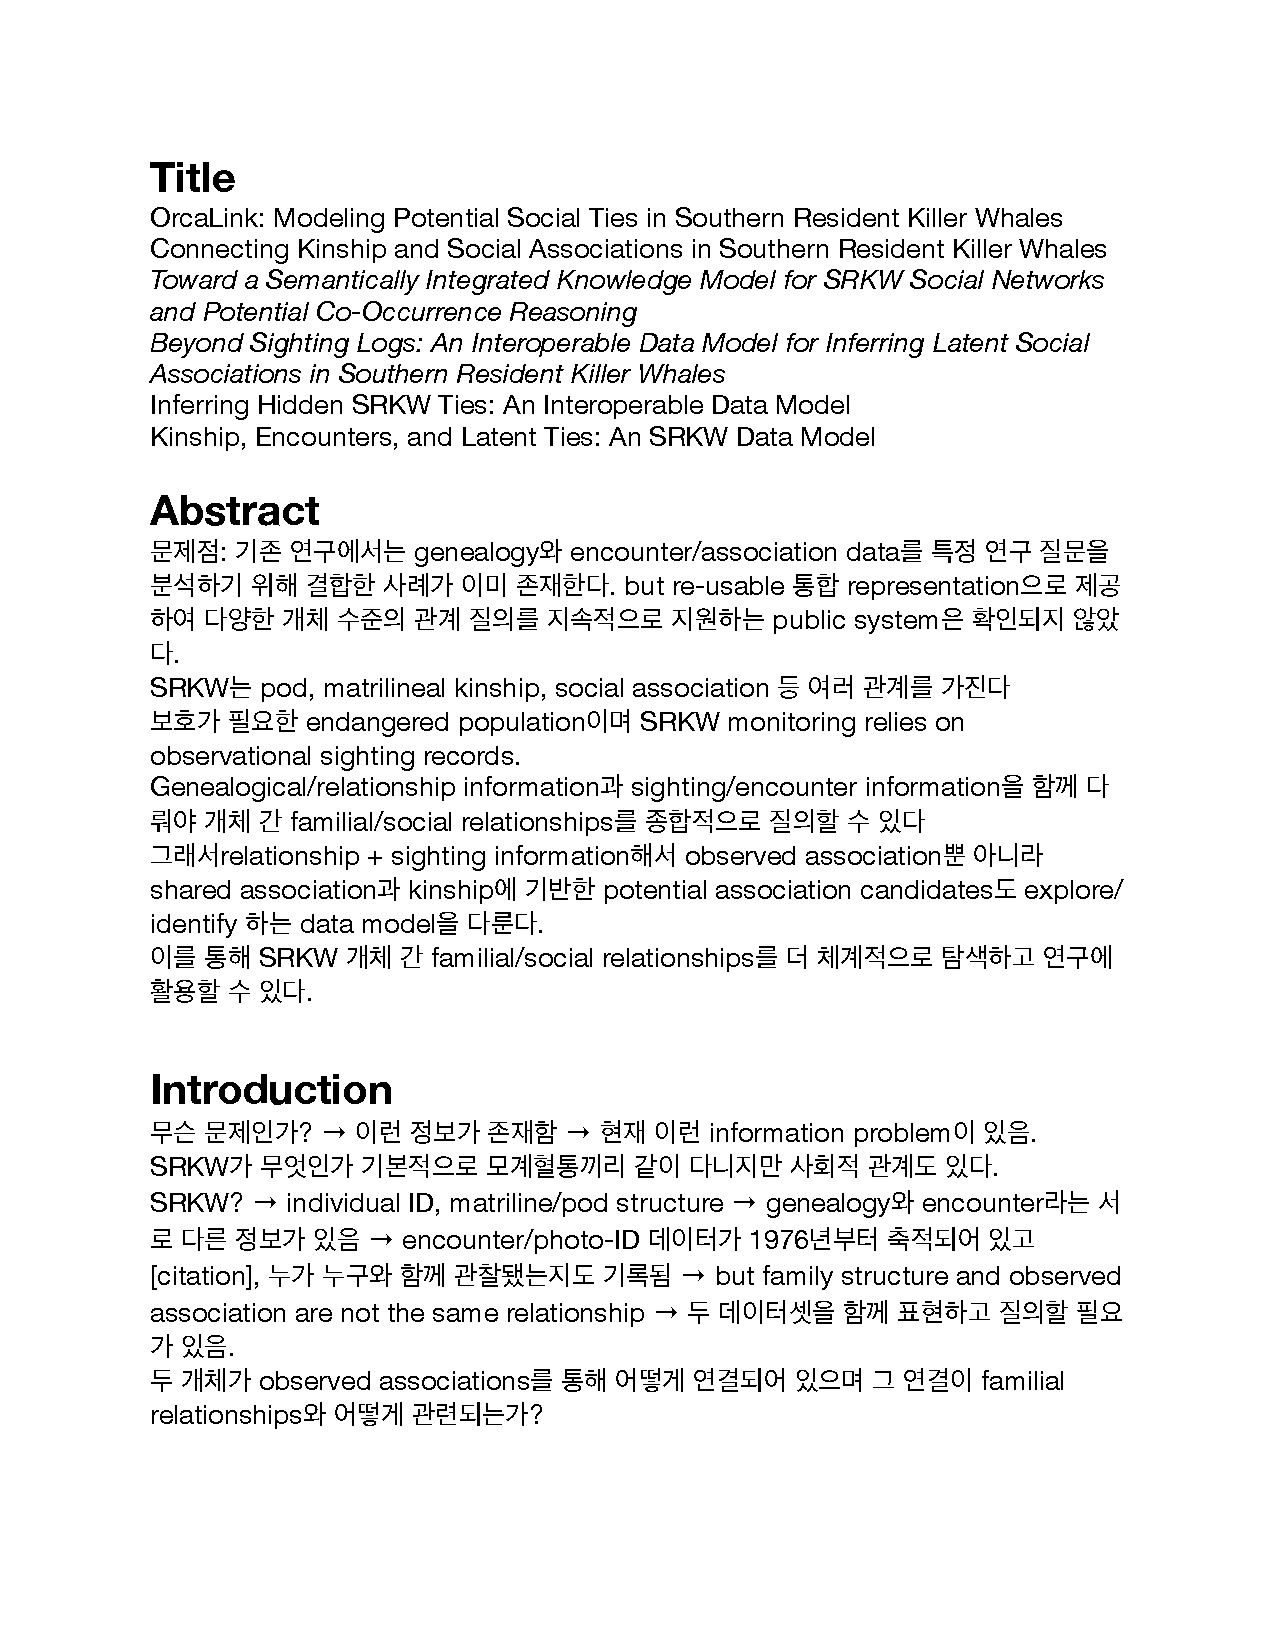
\includepdf[pages=-]{Proposal_Draft.pdf}

\end{document}


\endinput
%%
%% End of file `sigconf.tex'.